\documentclass[10pt]{article}
\usepackage{graphicx} % Required for inserting images
\usepackage{subcaption}
\usepackage{float}
\usepackage[T1]{fontenc}
\usepackage[utf8]{inputenc}
\usepackage{lmodern}
\usepackage[english]{babel}
\usepackage[autostyle]{csquotes}

\usepackage{comment}

\usepackage[backend=biber,style=authoryear]{biblatex}
\addbibresource{bibliography.bib}

\title{Image Classification on Satellite Imagery For Sustainable Water Harvesting Placement in Indigenous Communities of Northern Tanzania}
\author{Roshan Taneja, Yuvraj Taneja}
\date{\today}

\begin{document}

\maketitle

\begin{abstract}

In the remote regions of Northern Tanzania, women and children of the Maasai Tribe walk nine hours a day to collect water for their families. Over four years, our collaborative efforts with the Maasai communities have led to installing four water harvesting units, enhancing the local socio-economic conditions by facilitating educational opportunities and economic pursuits for over 4,500 individuals within a 10-mile radius.

This project presents a novel approach to addressing this issue by integrating satellite data and image classification to identify densely populated areas marked by uniquely shaped Maasai homes lacking a water supply and strategizing the placement of rainwater harvesting units. The backbone of this project was developing an image classification model trained on 10,000 hand-selected satellite image samples of Bomas. This model generated a density heatmap, enabling the strategic placement of water harvesting units in the most critical locations to maximize impact.

Our findings underscore the potential of satellite technology in humanitarian interventions, particularly in harder-to-reach areas where traditional surveying and data collection techniques are impractical. By leveraging remote sensing observations, we demonstrate a scalable and efficient solution for improving water accessibility in remote communities.
    
\end{abstract}

% ------------------------------------------------------------------------------------

\section{Introduction}

\subsection{Background and Context}

According to the United Nations, one in four people cannot access clean water(\autocite{United_Nations}). One such community is the Maasai in the Monduli District of Tanzania. They walk over nine hours per day to fetch water and face challenges due to climate change and land deforestation. Floods and droughts are more frequent and severe, and traditional water sources, such as rivers and springs, dry up. Annual rainfall in Tanzania is equal to or higher than US, yet they face challenges in accessing water. The community has been deploying water harvesting units along the main highway, which currently helps less than 4000 people, but only for short periods. The impact of even one water harvesting unit has been validated. The challenge is that over 30,000-40,000 Maasai live across hundreds of square miles with no highways and infrastructure like electricity or water. We need a better technique to identify the living locations, assess the density, and pick the right water harvesting solution that balances cost, ease of deployment, and sustainability. This paper takes the first step in identifying the living locations across hundreds of square miles using satellite images, machine learning, and image classification models. If this approach has high precision, it can be expanded to many regions for water resource planning and management opportunities.  There is a need for sustainable water management solutions to support communities like the Maasai and other regions in Africa.

\begin{figure} [H]
    \centering
    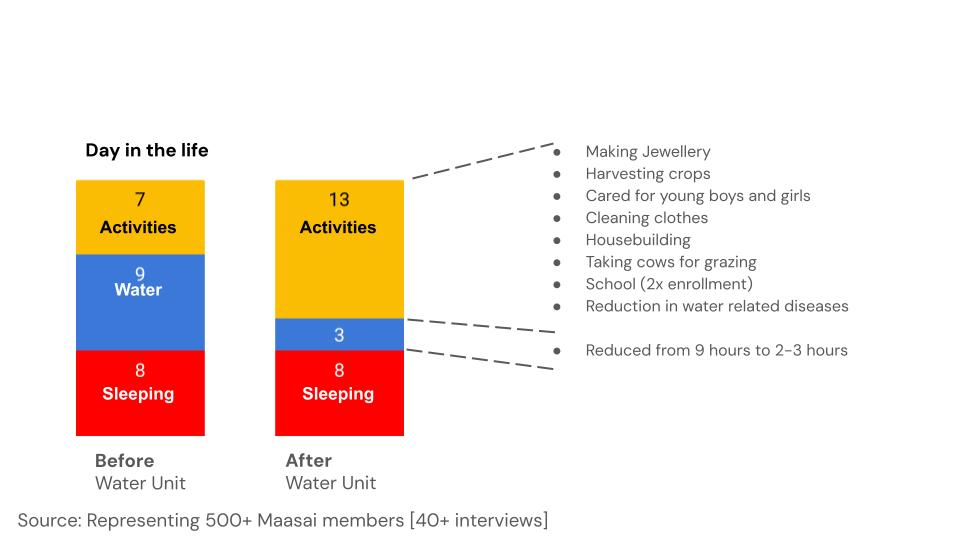
\includegraphics[width=1\linewidth]{images/beforeandafterwhu.jpg}
    \caption{Before and after the Water Harvesting Unit: Doubled the time spent on economic, social, and agricultural activities}
    \label{fig:bef_aft_results}
\end{figure}

The first water harvesting unit of 100K liters had a direct impact on the community. Specifically, kids have started coming to school more often and there is higher enrollment of students. Women have seen reduced time spent walking to fetch water and are using the extra time for social, agriculture and economic activities. Reduced walking from nine hours a day to two hours a day (Fig~\ref{fig:bef_aft_results}). 

(Fig~\ref{fig:bef_aft_results}). Given the impact, multiple additional projects have been executed include deploying a 30+K liter solutions serving the Nanja village and a water filtration system in Engirgiri that makes water collected in man-made pond that catches rainwater clean for use by the local community of Maasai.

\subsection{Problem Statement and Rationale}

% This isn't a problem statement

To support water harvesting solutions for 30,000-50,000 Maasai, we needed to identify the best places to locate them across 300-500 square miles. We can identify the best water harvesting solutions based on the population's density distribution. However, the government does not provide accessible maps of the Maasai's location. To design and plan solutions at scale, we decided to see if we could use satellite images and image classification to create a population map and validate the maps with local community involvement. The next step would be identifying the best locations for placing the water harvesting solutions.



% In Northern Tanzania, the Maasai community faces a severe challenge in accessing clean and safe water due to the arid climate and inadequate water infrastructure. This region, spanning thousands of square miles, predominantly relies on traditional water sources like rivers and springs, which are increasingly unreliable due to climate change and government intervention. The unique living structures of the Maasai, known as "bomas," are typically circular or oval enclosures made from thorny bushes and are difficult to detect using standard remote sensing techniques. These bomas, housing between 10 to 100 individuals, often do not have direct access to water sources, exacerbating the daily struggle for water.

% To address this critical issue, our project leverages satellite data to detect these uniquely shaped Bomas across extensive areas. By using advanced image classification techniques, we can identify densely populated regions lacking sufficient water access. The data source includes high-resolution satellite imagery analyzed through a custom-developed image classification model trained on 10,000 hand-selected images of Maasai homes.

%The solutions proposed aim to optimize the placement of water harvesting units based on the identified needs and local geographical conditions. The options for enhancing water accessibility include large units for housing groups, such as installing communal rainwater harvesting units with capacities of 100,000 liters to serve large groups of bomas, ensuring a continuous water supply for several days. Small Units on a Per-Boma Basis: Smaller, individual water collection systems for single bomas or small clusters provide a more personalized water management approach.Man-made Ponds and Dams: Creating larger-scale rainwater collection systems such as ponds or dams to benefit entire communities, especially in more densely populated areas.

% This comprehensive approach aims to provide immediate relief from water scarcity and contribute to the long-term sustainability of the Maasai way of life by integrating modern technology with traditional living patterns. The expected outcomes include reduced time spent collecting water, improved health and hygiene, and enhanced economic and educational opportunities for the community.

\subsection{Scope and Limitations}

We will limit our study to a small selected area of about 250 sq. miles. In addition, we will make limited modifications to the base computer vision algorithm we use. These limitations allow us to use a rapid iterative process to finalize the correct training data and algorithms. There are also other limitations in the data that we are using.

\subsubsection{Unique Structure and Materials of Bomas}

\begin{figure} [H]
    \centering
    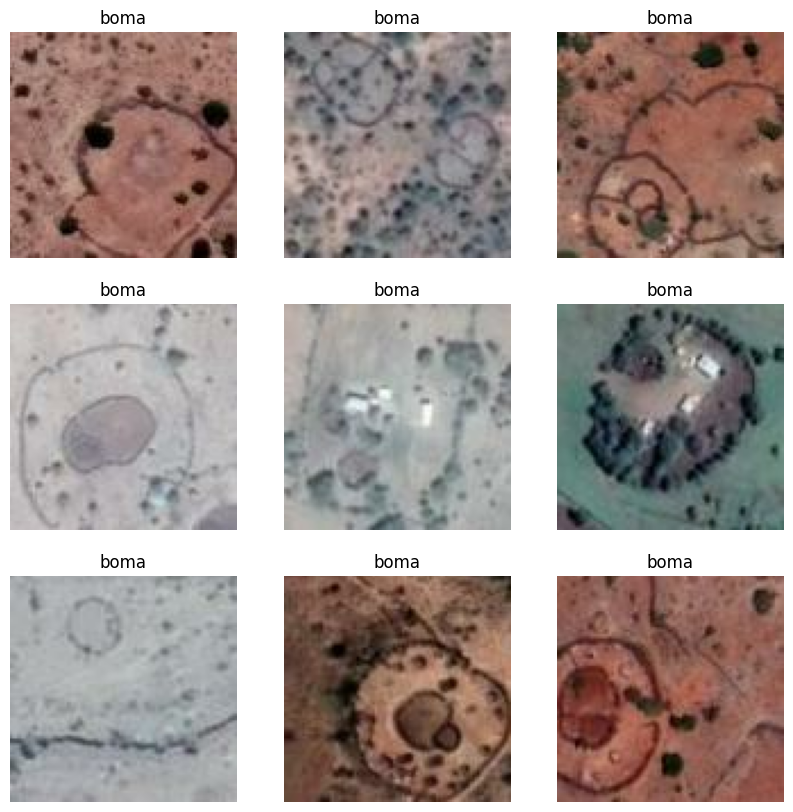
\includegraphics[width=0.8\linewidth]{images/types of bomas.png}
    \caption{Example of Variation in Landscape, Vegetation and Structure}
    \label{fig:types_of_bomas}
\end{figure}

Due to their polygamous nature, familial groups live together in large units called "Bomas." 

A Boma is a unique structure that is difficult to classify. There is no precise size to a Boma, but it usually consists of multiple small huts, a section for keeping goats and cows safe at night. There are a few characteristics that define a Boma. An outer barrier, usually made from rough bushes. Inside, there may be trees or other structures, such as shelters. At the center will be a smaller circle, also created with bushes, where cattle stay. These Bomas can house 10 to 50 people and sometimes be squares or other shapes, even open ones. Families who own cattle create an inner or outer circle or circles with other things, such as trees. Another issue is the contrast of the bushes with the environment, sometimes not showing up. (Fig~\ref{fig:types_of_bomas})


\subsubsection{Techniques Considered}

In evaluating three different methods for our project, we considered YOLOv7, OpenCV, and TensorFlow. YOLOv7, though highly optimized for speed and accuracy with minimal background detection errors, presented significant challenges. It proved difficult to integrate with Jupyter notebooks(\autocite{s23135849}). It performed inadequately with objects of varying sizes and shapes—critical for our project—and suffered from limited community support(\autocite{IJERTV10IS060287}), maintained by a small team. While boasting extensive community support and customizable settings, OpenCV was deemed overly complex for our beginner-level proficiency, featuring a steep learning curve(\autocite{9174593}).

Conversely, TensorFlow appeared as the optimal choice, balancing accessibility as an open-source tool and compatibility with Python and JavaScript, which is crucial for integrating with Google Earth Engine (GEE).
Despite its higher resource consumption and slower performance, TensorFlow's regular updates and new features make it the most suitable framework for our needs. It provides the necessary tools and support for successful project execution.

\subsection{Objectives}

This research project aims to optimize the placement of water harvesting solutions based on population density and natural water sources. To generate a population density map, we want to use satellite data to detect these uniquely shaped Bomas across selected regions. This data will help identify critical locations for deploying the appropriate water solutions. The options for enhancing water accessibility include large units for housing groups, such as installing communal rainwater harvesting units to serve large groups of Bomas and creating larger-scale rainwater collection systems, such as ponds or dams, to benefit entire communities, especially in more densely populated areas.

% ------------------------------------------------------------------------------------

\section{Methods}
\label{methods}

\subsection{Data Collection and Augmentation}
\label{data}

We considered two different sources for our training data. One was the Copernicus Institute website for the Copernicus Satellites and Google Earth Engine (GEE). We settled on GEE because writing a script to generate the training data from just a few points on a map was easier. We started with 2000 photos of Bomas and 500 photos of the environment (Omits a Boma). The accuracy was around 30\%, far below the required standards. The model needed help with a few problems. First, The color of the Boma circle blended in too well with the environment. Second, There wasn’t enough data to train the AI.

We realized that the images could be superimposed, meaning we could rotate and flip them to create more training data for the model. Using this new information, we generated 6,000 more photos of Bomas and 1500 more images of the environment. With this new model trained at 10,000, the accuracy skyrocketed to 93\%. Because these "Bomas" are often disguised and varied, more training would not increase the accuracy further. The model plateaus with the current constitution at a certain point due to the extreme shape, color, and size variation. Toggling with filters, cropping, grayscale, or increasing the contrast did not impact the accuracy. Perhaps more fine-tuning is necessary, but it's unlikely to change performance significantly.

\subsection{Training the Model}
\label{training}

We used a generic CNN model from the TensorFlow documentation for the model. We chose not to tune any hyperparameters or change any particular activation functions because we wanted to test the capabilities of the base model. Each Image is 100x100 with 3 color channels: Red, Green and Blue. The model takes in the image and outputs confidence in each class that it could be (Fig~\ref{fig:model_shape}).

\begin{figure} [H] % Put in diagram of the model
    \centering
    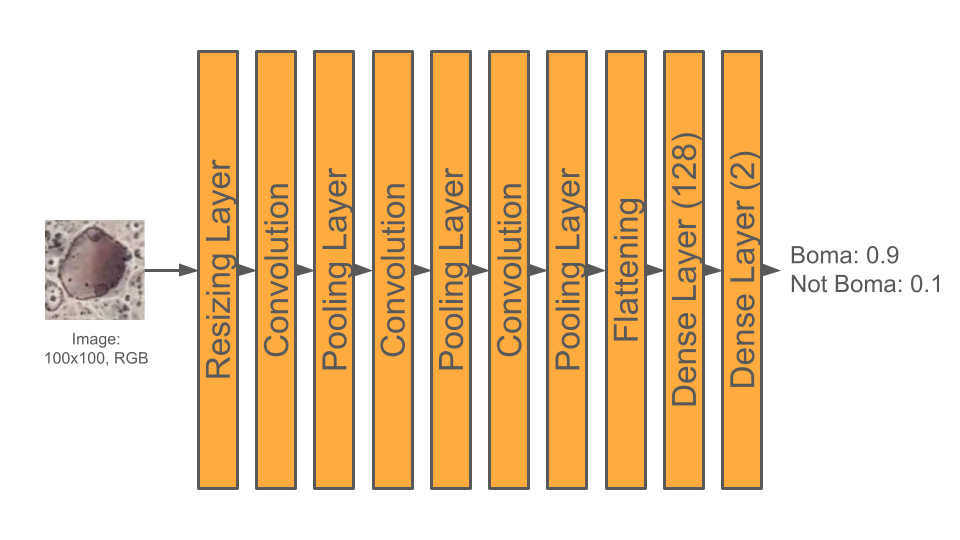
\includegraphics[width=1\linewidth]{images/Model Shape.png}
    \caption{Shape of the Model}
    \label{fig:model_shape}
\end{figure}

The model, in particular, is a generic CNN model that can classify objects with relatively minimal training. Here's a quick explanation of each layer's function in the model.

Rescaling layer: Rescale all the image values between 0 and 1 because working with smaller numbers makes the math for the model easier.

Convolutional Layers (Conv2d): it has three layers that apply filters to the image to highlight features like edges, textures, or patterns. In this case, it most likely filters for circular or closed shapes similar to the shape of the Boma.

MaxPooling Layers: After each Conv2d Layer, there's a pooling layer that reduces the size of the filtered image by only keeping the most prominent features in each small area. This makes the model faster and focuses on the most critical parts of the image.

Flattening Layer: After filtering and Pooling, the model flattens the data, turning the 2d filtered images into a long list of numbers. This prepares the data for the final classification.

Dense Layer: There are two “dense” layers. It takes the flattened Layer and transforms it through another “relu” layer, reducing it to 128 numbers. This helps in capturing relationships between filtered features.

Finally, the model takes the 128 numbers and outputs them into a final set of 2 scores: “percentage it is a Boma” and “percentage it isn't a Boma.”

\begin{figure}
    \centering
    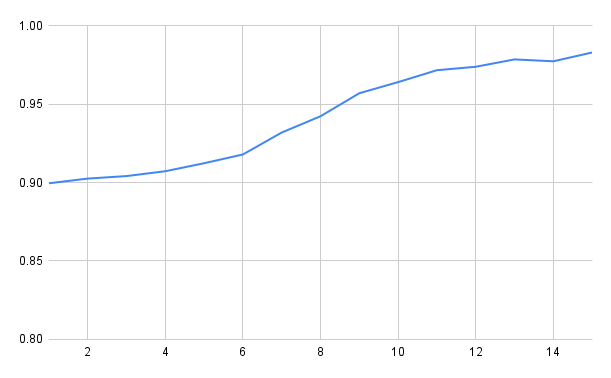
\includegraphics[width=1\linewidth]{images/Training Accuracy over 15 epochs.png}
    \caption{Training Accuracy over 15 epochs}
    \label{fig:Training_Accuracy}
\end{figure}

Trained for only 5 Epochs; 1 training cycle. After training the first time with 15 epochs, I noticed that the accuracy seems to plateau around 97\% (Fig.~\ref{fig:Training_Accuracy}). Therefore, for future training, the model was limited to 10 epochs.

\begin{table} [H]
    \centering
    \begin{tabular}{rrrl}
    \multicolumn{1}{c}{\textbf{Epoch}} & \multicolumn{1}{c}{\textbf{Training Loss}} & \multicolumn{1}{c}{\textbf{Training Accuracy}} &  \\
    1  & 0.3279 & 0.8995 &  \\
    2  & 0.3031 & 0.9025 &  \\
    3  & 0.2801 & 0.9041 &  \\
    4  & 0.2526 & 0.9072 &  \\
    5  & 0.2267 & 0.9123 &  \\
    6  & 0.1942 & 0.9179 &  \\
    7  & 0.1612 & 0.9319 &  \\
    8  & 0.1353 & 0.9423 &  \\
    9  & 0.1091 & 0.957  &  \\
    10 & 0.091  & 0.9641 &  \\
    11 & 0.075  & 0.9717 &  \\
    12 & 0.0653 & 0.9739 &  \\
    13 & 0.0543 & 0.9786 &  \\
    14 & 0.0546 & 0.9774 &  \\
    15 & 0.044  & 0.983  & 
    \end{tabular}
    \caption{Raw data from Training for 15 epochs}
    \label{tab:training_raw_data}
\end{table}


% ------------------------------------------------------------------------------------

\subsection{Procedure}
\label{procedure}
% Deploying the model?

Google Earth Engine (GEE) enables an image processing technique called "Image Stacking." Typically, These stacks would allow users to perform time-series analysis, detect trends, and monitor environmental changes using satellite imagery and other geospatial data. However, there is a lesser-known technique in which the user "squashes" the highest-resolution sections together to generate exceptionally high-resolution content to read. This can be useful, especially for filling holes in scanning, removing lower-resolution mapping, or avoiding cloudy content. 

We specified a sample of the Monduli district of just over 260 square miles (Fig~\ref{fig:designated_area}) and isolated it for recent times in the last four weeks (2024-02-01 to 2024-02-29). We manually went through the images and isolated them with virtually no cloud coverage over the selection area (I found out later that the GEE API allows you to identify "CLOUDY\_PIXEL\_PERCENTAGE.")

\begin{figure} [H]
    \centering
    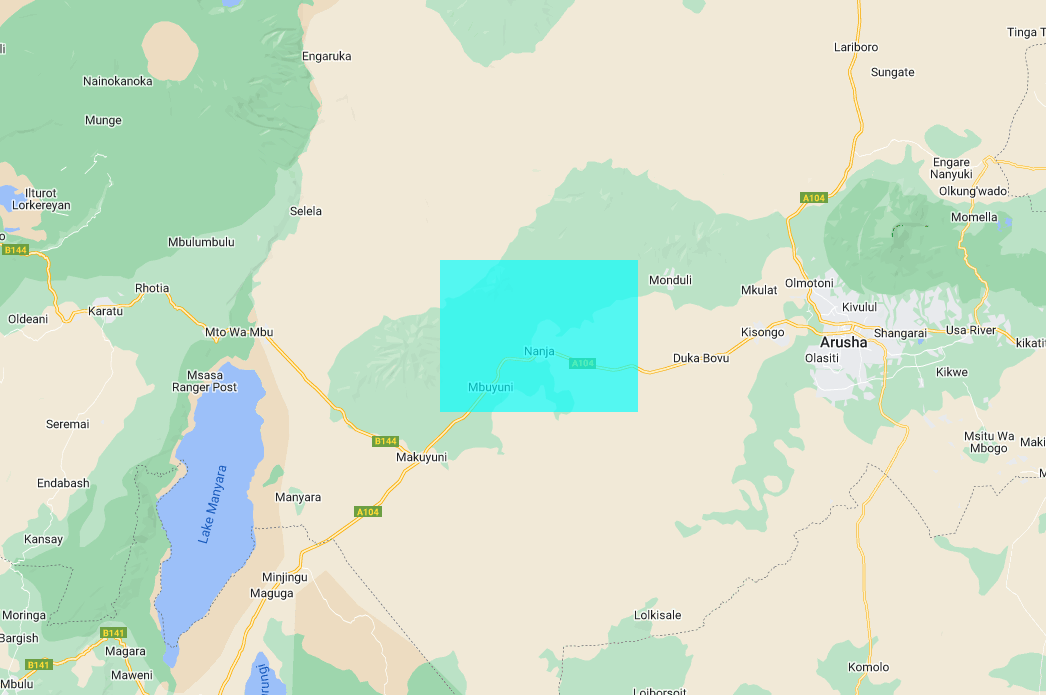
\includegraphics[width=1\linewidth]{images/studyarea.png}
    \caption{Designated Area for First Test, 260 square miles between Serengeti and Arusha}
    \label{fig:designated_area}
\end{figure}

We took the image stack and filtered out all bands greater than 10-20 meters per pixel. For Copernicus/S2\_Harmonized, those included ['B2', 'B3', 'B4', 'B5', 'B6', 'B7', 'B8', 'B8A', 'B11', 'B12'] (Fig~\ref{fig:cop_bands_chart}). Then, we layered the images according to the variable importance GEE provided (Fig~\ref{fig:band_importance}). We created an image stack of all collected wavelengths of color light.

\begin{figure} [H]
    \centering
    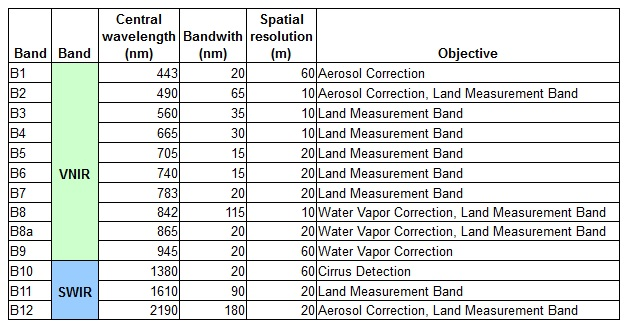
\includegraphics[width=1\linewidth]{images/copernicus_band_resolution.png}
    \caption{Band Resolutions Provided by Copernicus}
    \label{fig:cop_bands_chart}
\end{figure}

\begin{figure} [H]
    \centering
    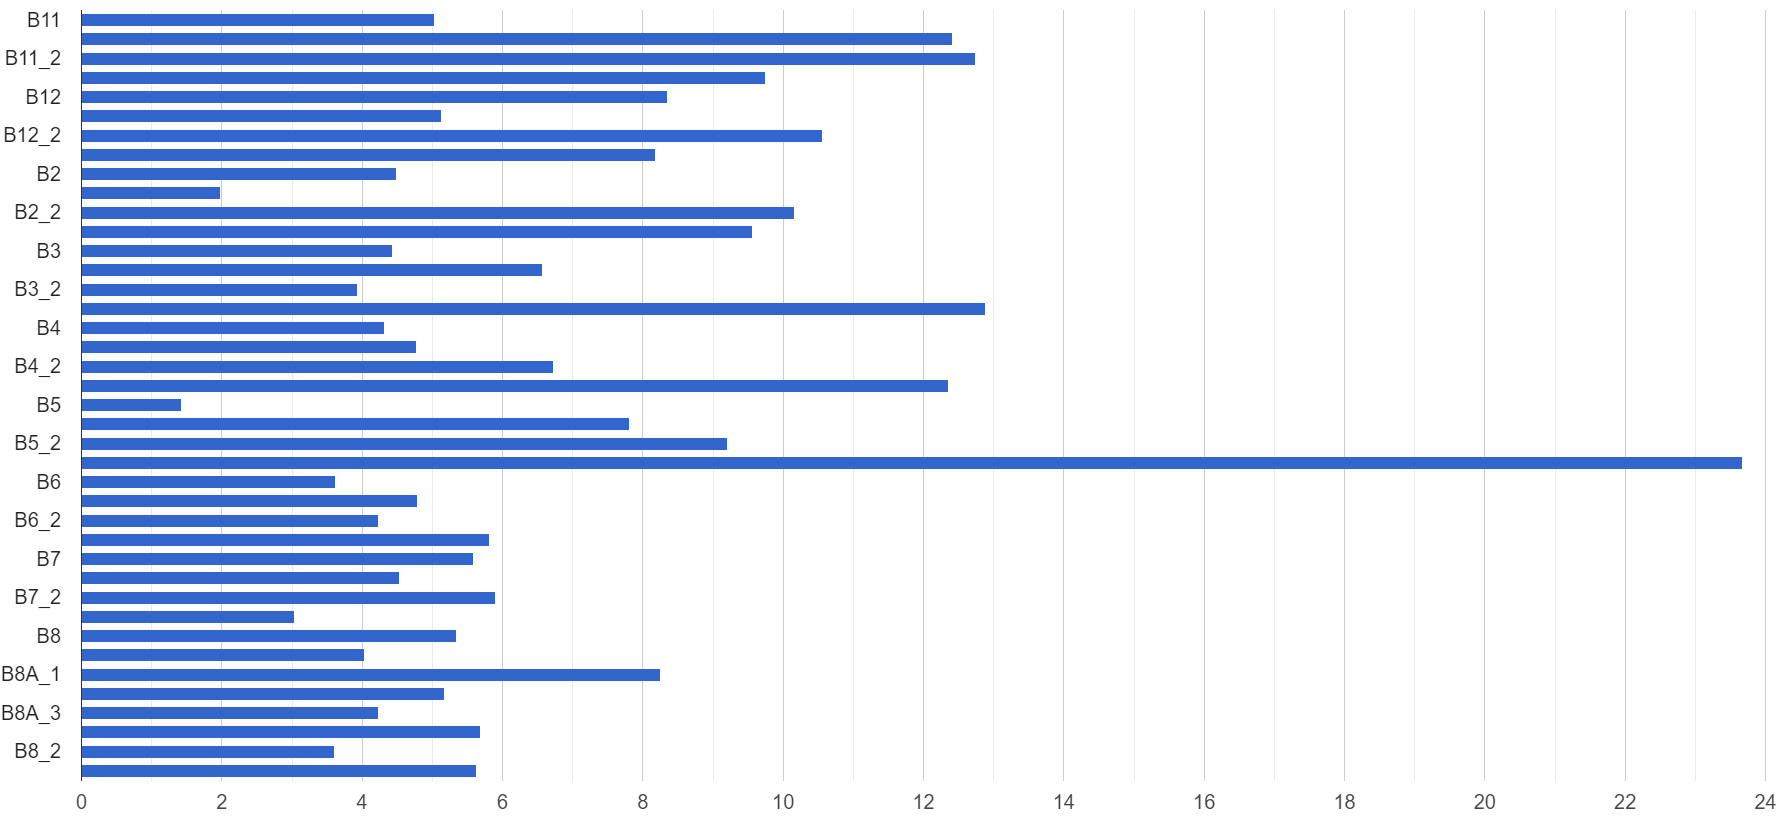
\includegraphics[width=1\linewidth]{images/bands importance.png}
    \caption{Variable Band Priority}
    \label{fig:band_importance}
\end{figure}

We separated the image stack into slices run individually through the model (Fig~\ref{fig:model_shape}). The final image stack was 10980 pixels by 10980 pixels. To classify some of these Bomas accurately, we would need to overlap the samples by a small portion for edge cases where a Boma would be too far into the border and missed by either selection. We settled for a 20-pixel overlap in both the horizontal and vertical directions.

% ------------------------------------------------------------------------------------

\section{Results}
% Green Dot converted into heatmap; Black small dots
% Discussion for location of water bodies/water harvesting units

It took over 4 hours to run the model discussed in section~\ref{training} over the selected area of 260 square miles on GEE. Everywhere the confidence of the model was above 80\%, the coordinates of that point were recorded (Fig~\ref{fig:OutputOnSample}). Figure~\ref{fig:OutputOnSample} displays a dot for each recorded sample plotted out by relative coordinate. In total, the model classified 488 Bomas over the selected area. We transposed the relative coordinates on top of the image stack of our designated area generated in section~\ref{procedure} (Fig~\ref{fig:OverlayedMap}). Figure~\ref{fig:OverlayedMap} displays all the classified Bomas relative to Nanja Dam (natural reservoir).

\begin{figure} [H]
    \centering
    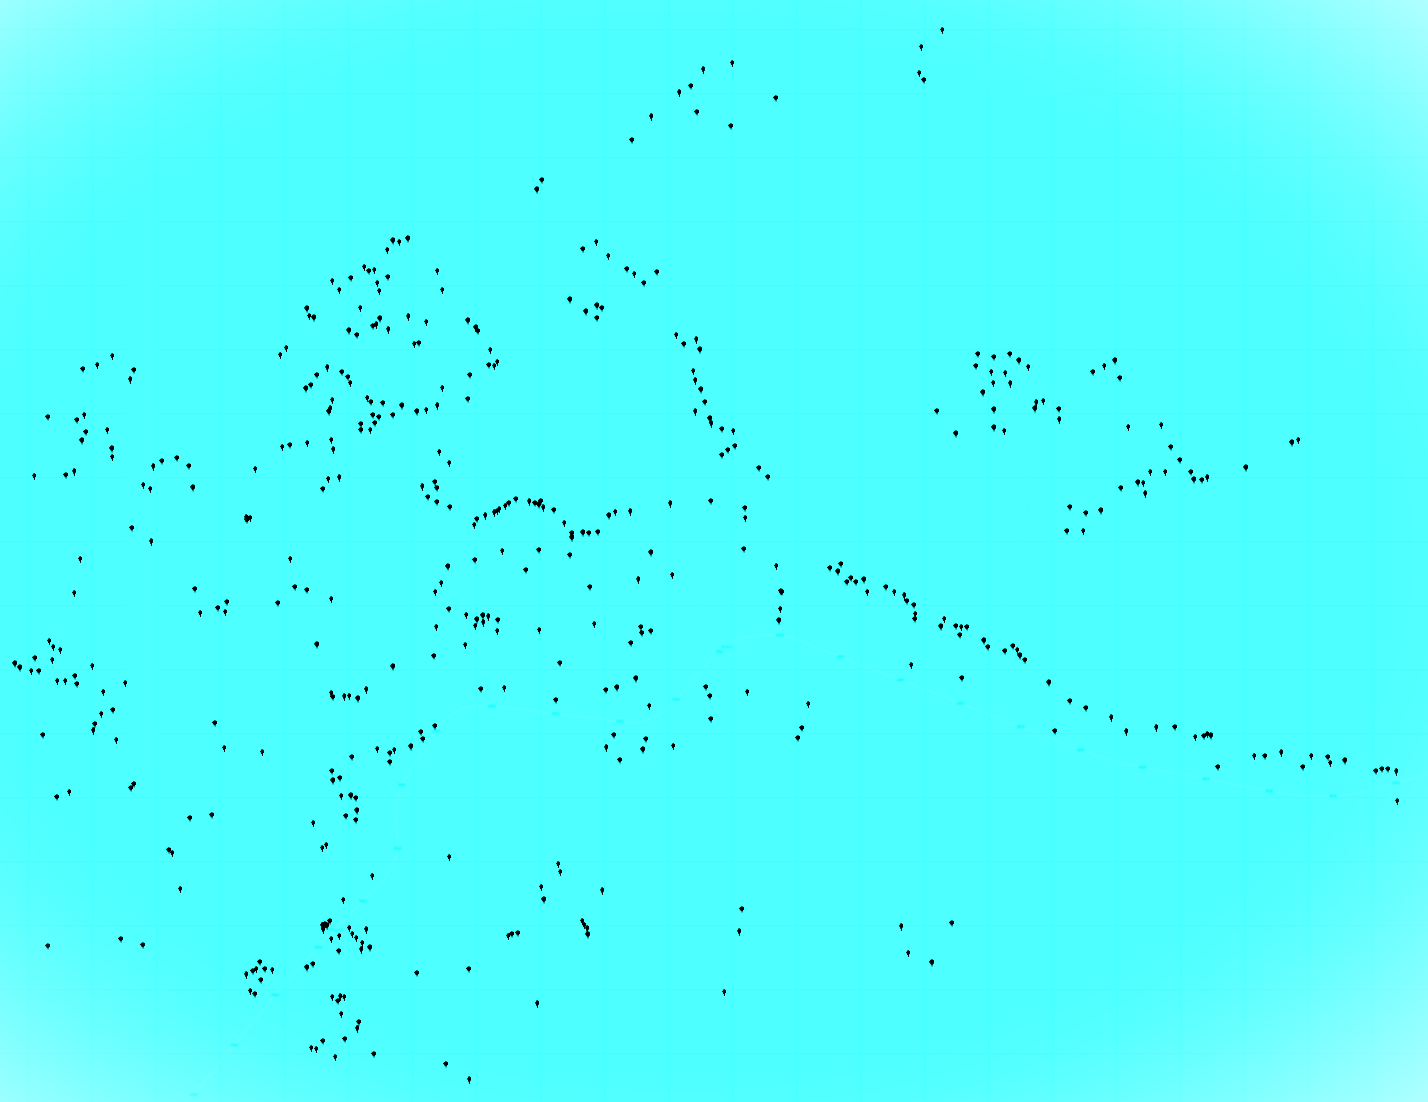
\includegraphics[width=1\linewidth]{images/cv_output.png}
    \caption{Output with relative coordinates}
    \label{fig:OutputOnSample}
\end{figure}

\begin{figure} [H]
    \centering
    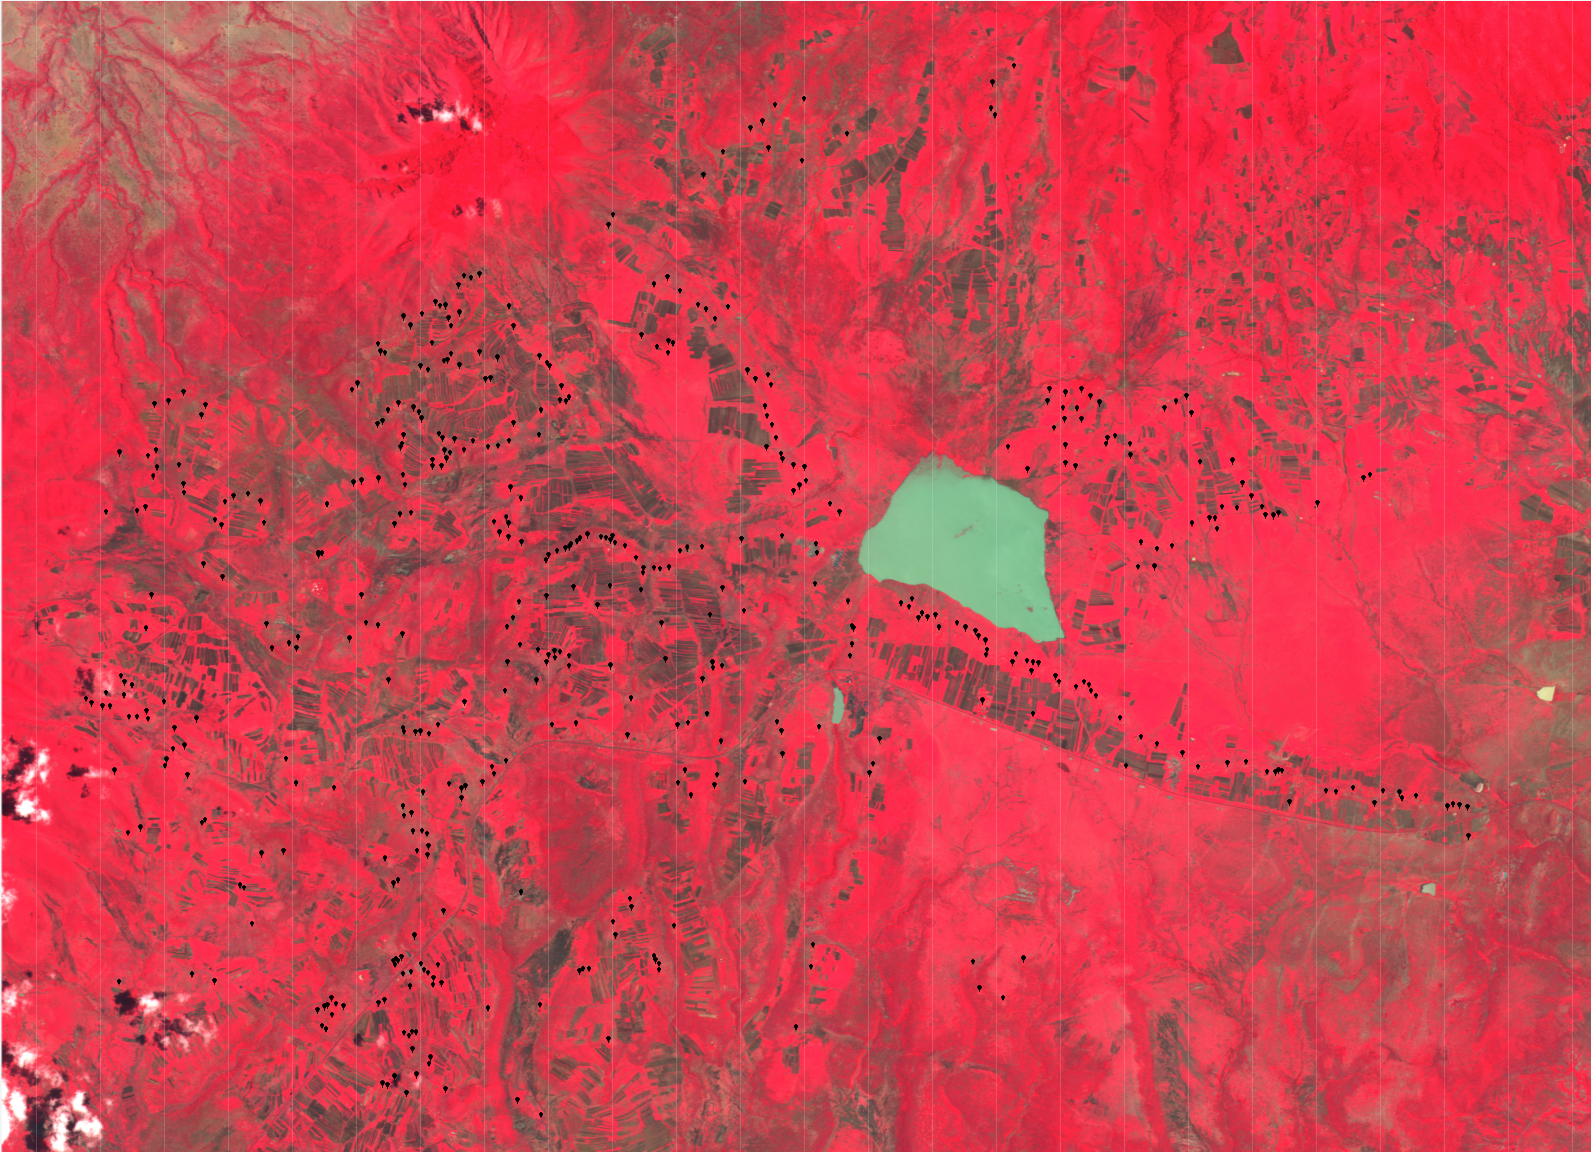
\includegraphics[width=1\linewidth]{images/Outputoverlayrealmap.png}
    \caption{Output Overlayed Over Image Stack}
    \label{fig:OverlayedMap}
\end{figure}

% ------------------------------------------------------------------------------------

\section{Discussion}

\subsection{Key Findings}

We can see that large populations seem to live in dense communities of several dozen Bomas (A, B, F, J, K). They also live in lines along the edges of major geological formations such as dried riverbeds or reservoirs (C, E, G). In addition, it also looks like many communities reside parallel to the major highway that runs through the area (H, I). We can use this information to isolate large communities and identify the best locations for rainwater harvesting solutions (Fig~\ref{fig:Communities and Major Highway}).

\begin{figure} [H]
    \centering
    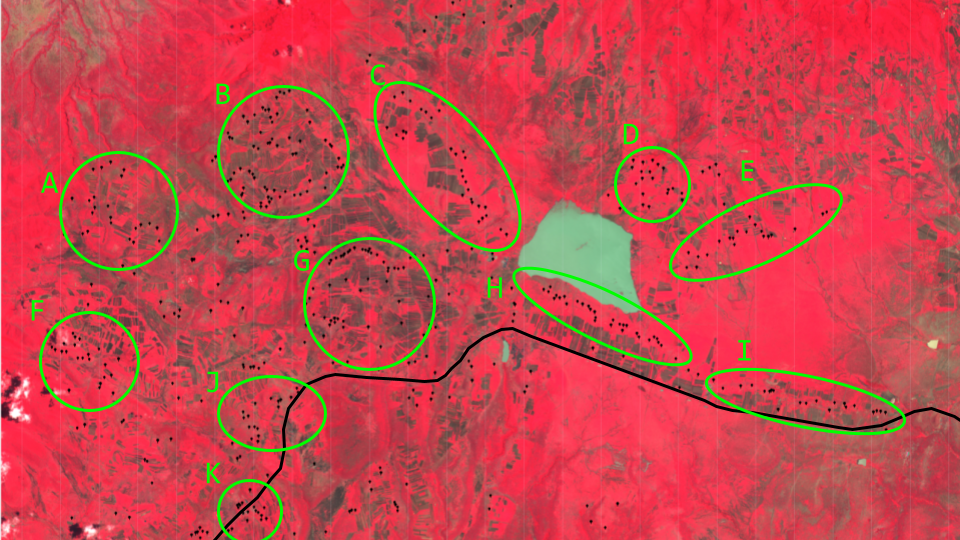
\includegraphics[width=1\linewidth]{images/Communities and Highway Highlighted.png}
    \caption{Large High-Density Community Collections of Bomas Highlighted with Major Highway}
    \label{fig:Communities and Major Highway}
\end{figure}

Larger groups, especially those further away from the Nanja Dam, such as A, B, and F, can be our project's starting point. We can identify locations within these more prominent groups to place these water harvesting solutions. 

\subsection{Limitations of Outputs}

As you can see in the zoomed-in photos, the images streamed to the web editor are very low quality from the perspective of the GEE editor. However, there are noticeable patterns where the model "identified" Bomas (Fig~\ref{fig:Zoomed_Overlayed}). A quick look at the coordinates in Google Maps (with higher resolution but dated images) shows that at least a couple of these points seem to be housing units. However, many Bomas seem not identified (Fig~\ref{fig:zoomed_google_maps}), or only large, easily identifiable with thick or dark boundaries are identified.

\begin{figure} [H]
    \centering
    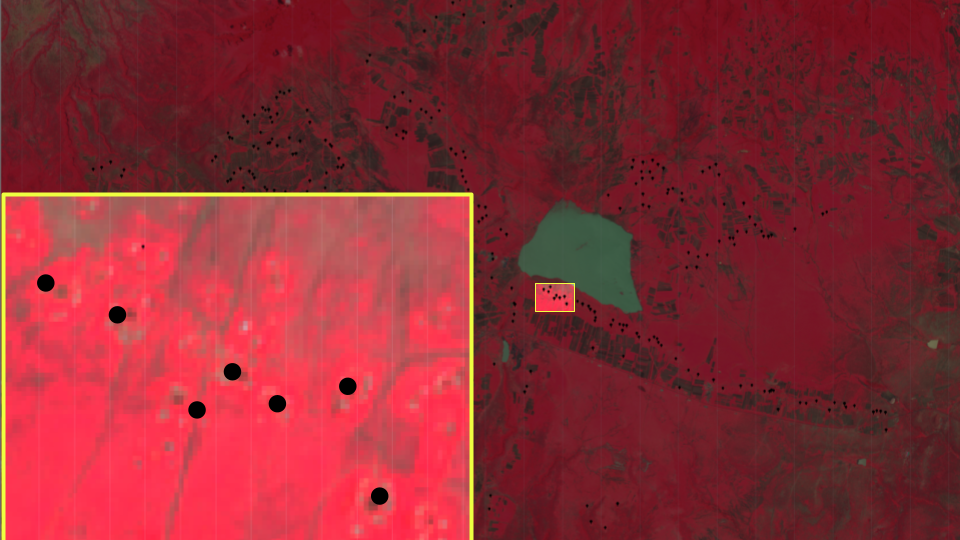
\includegraphics[width=1\linewidth]{images/zoomed in overlay.png}
    \caption{Zoomed In Portion on GEE}
    \label{fig:Zoomed_Overlayed}
\end{figure}

\begin{figure} [H]
    \centering
    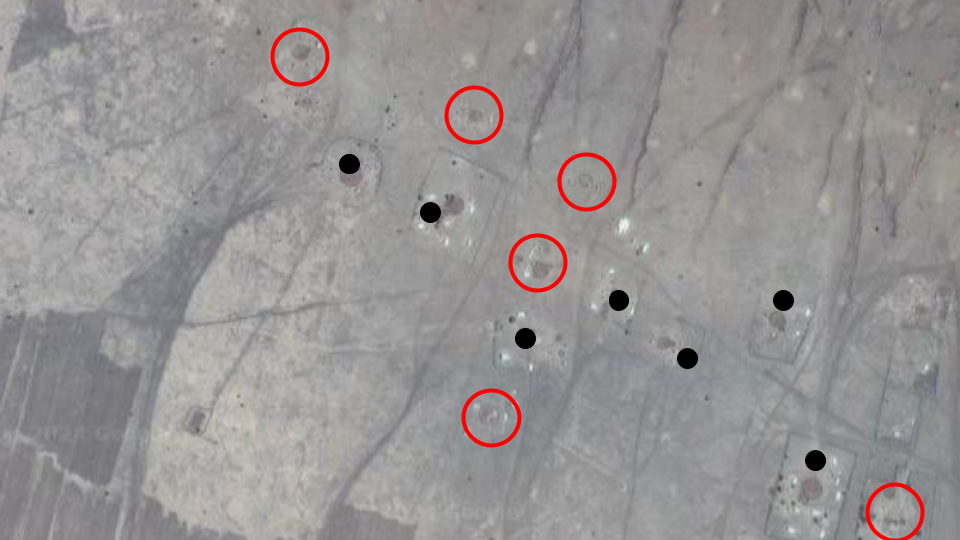
\includegraphics[width=1\linewidth]{images/zoomed google maps highlighted.png}
    \caption{Zoomed In Portion on Google Maps Displaying False Negatives}
    \label{fig:zoomed_google_maps}
\end{figure}

In addition, our training data may have also caused some of these inaccuracies. The dataset was very unbalanced, with 75\% of our data being photos of Bomas and only 25\% of our data being photos of the environment. The model may have been more accurate with a more balanced training set.

\subsection{Implications and Significance}

Maps like these can be used in numerous contexts, especially in other humanitarian efforts. Now that we understand the population locations better, we can use this data to structure other initiatives, like drone-based medical delivery, better road systems, or the locations of medical facilities. Other organizations, or even the Tanzanian Government, could use this data to better understand where their Indigenous populations are located.

\subsection{Community Involvement}

The local Maasai community is working with us to validate the outputs' results with a formal group of Maasai members from across the region. With the validated data, the next step is to segment the map into high-density, medium-density, and low-density clusters. Based on the size and area of the clusters, we can identify the best possible water access solutions.

We are evaluating three types of deployment solutions with the community. The first is a low-cost solution of 5000-liter tanks with rainwater harvesting at a Boma. This applies to distant Bomas, which are not close to any significant water access location. The second is a sizeable 100,000-liter water harvesting solution deployed for a set of Bomas together that will be helpful for large-density/medium-density regions. The third is a man-made pond/small lake where rainwater collects, and a solar-powered pump and filtration unit provide clean water access.

One of the core principles of ensuring long-term sustained impact and ownership is to empower and enable the local Maasai community to pick these solutions and invest their time in the planning, deployment, and ongoing maintenance. With over 480+ Bomas and 50000 Maasai, we will also need to support them in establishing a more structured Water Council that takes accountability for equitable water use and ongoing maintenance. This work is done with Maji Wells [Mbayani Tayai, local Maasai leader] and other local community leads.

% ------------------------------------------------------------------------------------

\section{Conclusion}

This study has demonstrated the potential of integrating advanced satellite imagery analysis with traditional water management practices to significantly enhance water accessibility for the Maasai communities in Northern Tanzania. By employing TensorFlow in conjunction with Google Earth Engine, we developed a model that identifies populations. These maps can optimize water solution placement, tailoring solutions to the region's unique geographical and social structure.

We have decided to move forward with a mix of individual and communal rainwater harvesting units in or near the locations.

Future efforts should focus on refining our models' predictive accuracy by incorporating more diverse data sets and real-time environmental monitoring. Additionally, exploring partnerships with local governments and international organizations will be crucial in scaling these solutions to other similarly affected communities globally. By continuously blending technology with traditional knowledge, we can foster more resilient communities that are better equipped to manage their natural resources sustainably.

\section*{Acknowledgement}

We thank Ananya Rao (Carnegie Mellon University) for mentoring and supporting this project and Mbayani Tayai for validating ground truths in Tanzania.

\printbibliography

\end{document}